\section{การทำงานร่วมกันระหว่าง HAPS และ Terrestrial Networks}

เทคนิค interference สามารถใช้เพื่อประสานการทำงานระหว่าง HAPS และ TN ได้
นั่นก็เพื่อ utilize ทรัพยากรทั้งบน HAPS และ TN ให้มากขึ้น
โดยรูปแบบของการประสานการทำงานนั้นเป็นไปตามรูปที่ \ref{fig:03-different-cases}

\begin{figure}[h]
\centering
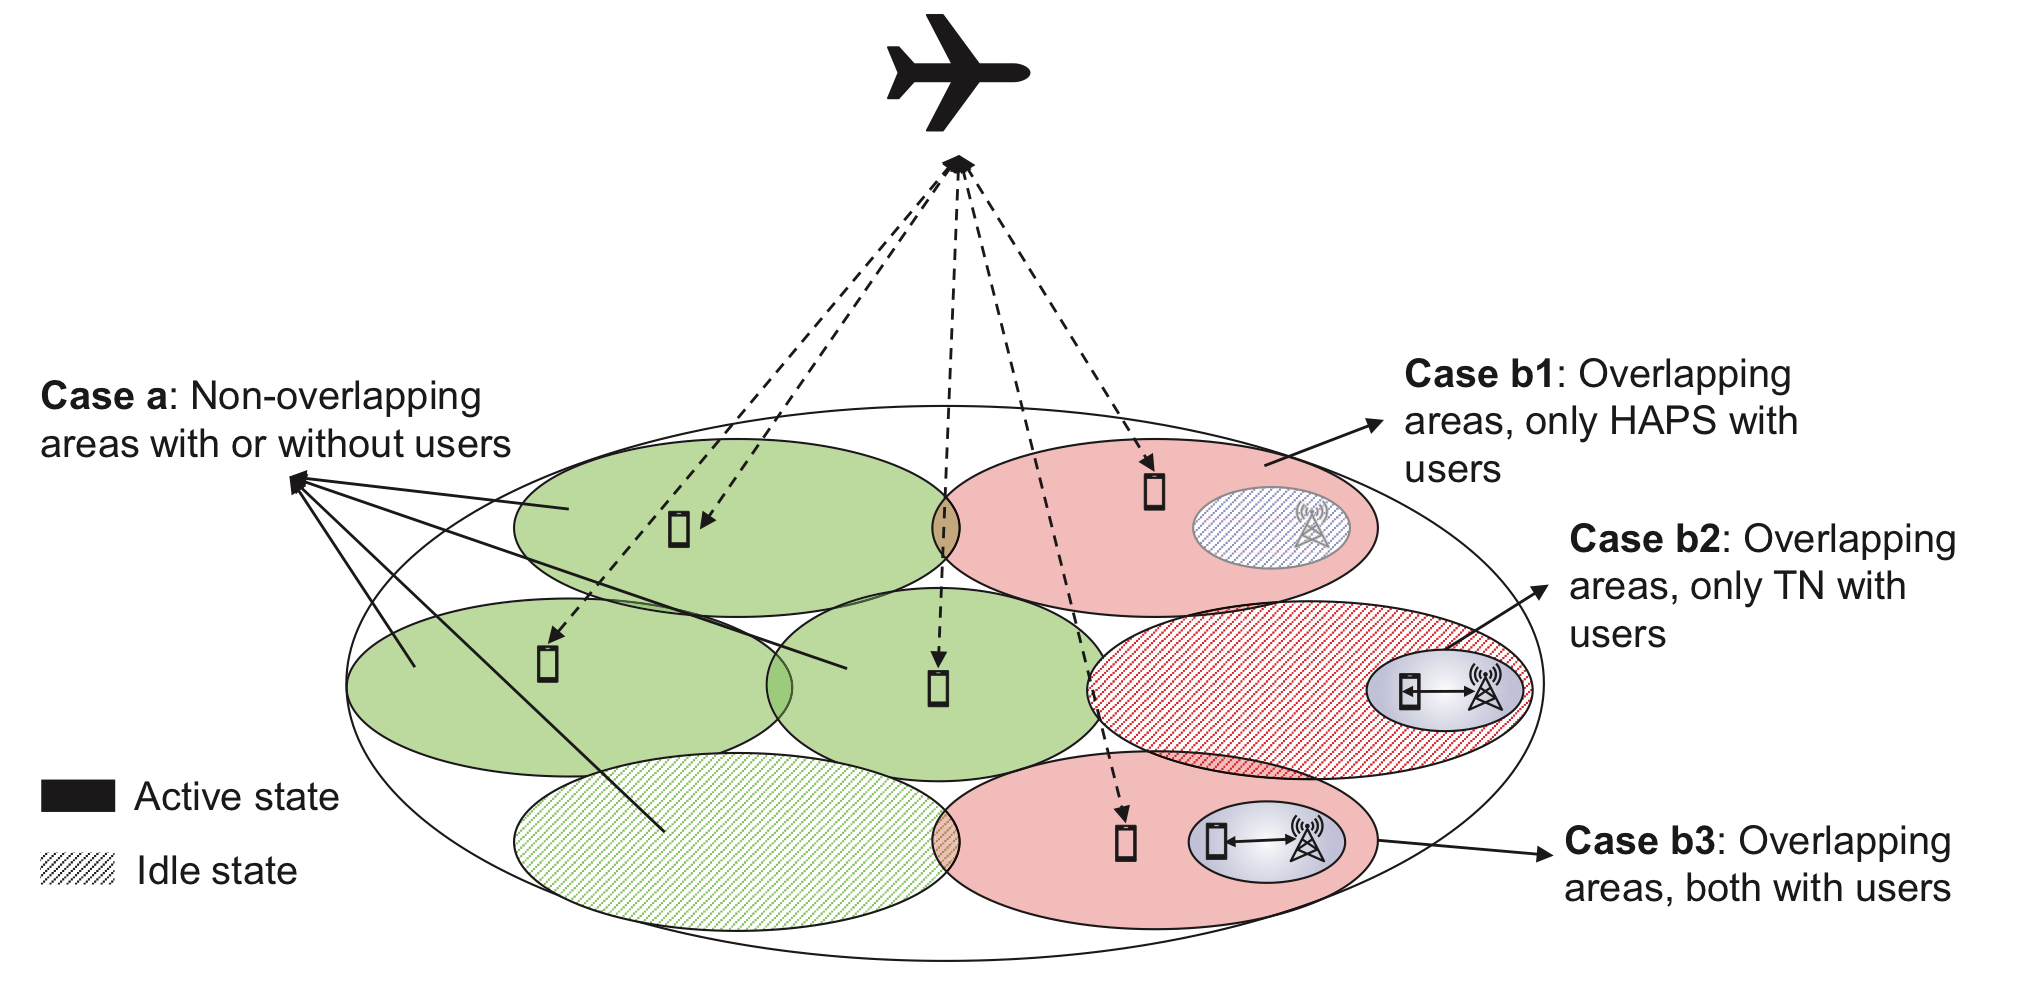
\includegraphics[width=0.7\textwidth]{03_different-cases.jpeg}
\caption[Different interference cases]{Different cases based on the traffic distribution and the deployment of integrated system} \label{fig:03-different-cases}
\end{figure}

หากพิจารณาการกระจาย traffic และความเป็นไปได้ในการที่จะมี TN ที่พร้อมให้ประสานการทำงานอยู่ใน coverage area
จะสามารถแบ่งการทำงานได้เป็นหลายกรณี ดังต่อไปนี้

\subsection{Non-overlapping Areas (Case a)}

กรณีที่มีเฉพาะ HAPS เท่านั้นที่ให้บริการใน coverage area

\subsection{Overlapping Areas Between HAPS and Terrestrial Coverage (Case b)}

กรณีที่มีทั้ง HAPS และ TN อยู่ใน coverage area ซึ่งในกรณีนี้จะต้องพิจารณาความพร้อมในการให้บริการของทั้ง
HAPS และ TN โดยสามารถแบ่งแยกเป็นกรณีย่อยได้ดังนี้

\begin{description}
    \item[Traffic only in HAPS system (Case b1)] HAPS ที่ทำงานเพื่อให้บริการ coverage area และ TN base station ใน coverage area นั้นอยู่ห่างไกลกัน
เนื่องจากไม่มี traffic เกิดขึ้นใน TN base stations จึงสามารถตั้งเป็นสถานะ idle ได้เพื่อประหยัดการใช้พลังงาน
และลด interference ระหว่าง HAPS และ TN
    \item[Traffic only in TN (Case b2)] ไม่มี traffic เกิดขึ้นใน HAPS ใน coverage area และไม่เกิด interference จาก HAPS ไปสู่ TN ใน coverage area
แต่ยังคงต้องพิจารณา interference จาก HAPS อื่น ๆ
    \item[Traffic only in both HAPS and TN (Case b3)] เกิด interference ทั้งจาก HAPS อื่น ๆ และระหว่าง HAPS กับ TN ใน coverage area
ซึ่งเป็นสาเหตุให้จะต้องออกแบบการประสานการทำงานระหว่าง HAPS และ TN อย่างระมัดระวัง
\end{description}
